\documentclass[tikz, multi=tikzpicture, margin=5mm]{standalone}
\usepackage{amsmath}

% --- Colors matching the python script & blog post math ---
\definecolor{Ocol}{HTML}{3273F6}    % Ray Origin (Blue)
\definecolor{Dcol}{HTML}{FF4B4B}    % Ray Direction (Red)
\definecolor{Ccol}{HTML}{109618}    % Sphere Center (Green)
\definecolor{Rcol}{HTML}{990099}    % Radius (Purple)
\definecolor{Acol}{HTML}{FF9900}    % Triangle Vertex A (Orange)
\definecolor{Bcol}{HTML}{0099C6}    % Triangle Vertex B (Light Blue)
\definecolor{Ctri}{HTML}{DD4477}    % Triangle Vertex C (Pink)
\definecolor{Textcol}{HTML}{333333}
\definecolor{Gridcol}{HTML}{E0E0E0}

\usetikzlibrary{calc, intersections, arrows.meta, positioning}

\tikzset{
    >=Stealth,
    font=\sffamily
}

\begin{document}

% ---------------------------------------------------------
% 4. Ray-Triangle Intersection (Möller-Trumbore)
% ---------------------------------------------------------
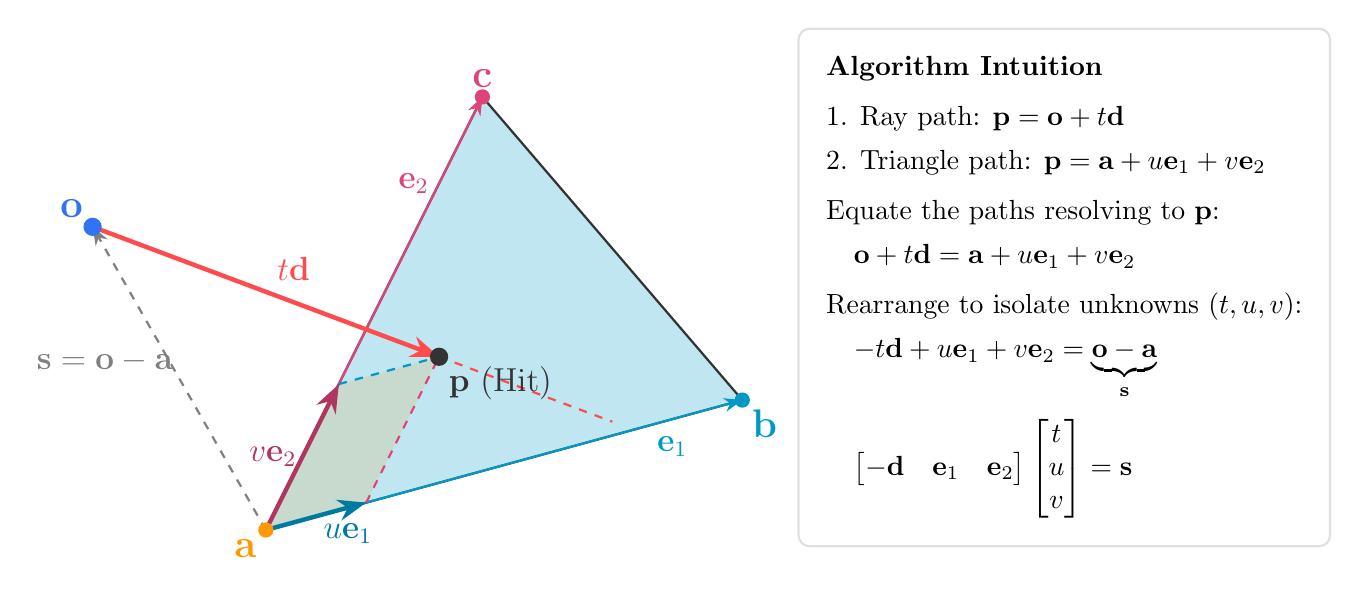
\begin{tikzpicture}[scale=1.1]
    % Grid
    % \draw[step=1, Gridcol, very thin] (0,0) grid (10,8);
    
    % Coordinates
    \coordinate (A) at (2.5, 2);
    \coordinate (B) at (8, 3.5);
    \coordinate (C) at (5, 7);
    \coordinate (O) at (0.5, 5.5);
    \coordinate (P) at (4.5, 4); % Intersection Hit point

    % Mathematically calculate u, v coordinates to make the parallelogram precise
    % P - A = (2, 2). e1 = (5.5, 1.5), e2 = (2.5, 5)
    % Resolving gives u ≈ 0.2105, v ≈ 0.3368
    \coordinate (ue1) at ($(A)!0.2105!(B)$);
    \coordinate (ve2) at ($(A)!0.3368!(C)$);

    % Draw Triangle Background
    \filldraw[fill=Bcol!25, draw=Textcol, thick] (A) -- (B) -- (C) -- cycle;

    % Draw the (u,v) parallelogram to visually explain the barycentric mapping
    \fill[Acol, opacity=0.15] (A) -- (ue1) -- (P) -- (ve2) -- cycle;

    % Vectors e1 and e2 (Full Edges)
    \draw[->, Bcol, thick] (A) -- (B) node[pos=0.8, below right, font=\large] {$\mathbf{e}_1$};
    \draw[->, Ctri, thick] (A) -- (C) node[pos=0.8, left, font=\large] {$\mathbf{e}_2$};

    % u*e1 and v*e2 (Scaled basis vectors)
    \draw[->, Bcol!80!black, ultra thick] (A) -- (ue1) node[midway, below right=-2pt, font=\large] {$u\mathbf{e}_1$};
    \draw[->, Ctri!80!black, ultra thick] (A) -- (ve2) node[midway, left=-2pt, font=\large] {$v\mathbf{e}_2$};

    % Dashed parallelogram projection lines
    \draw[dashed, Ctri, thick] (ue1) -- (P);
    \draw[dashed, Bcol, thick] (ve2) -- (P);

    % Vector s (Offset vector from vertex to ray origin)
    \draw[->, black!50, thick, dashed] (A) -- (O) node[midway, above left=-2pt, font=\large] {$\mathbf{s} = \mathbf{o} - \mathbf{a}$};

    % Ray line & direction (Scaled by t)
    \draw[->, Dcol, ultra thick] (O) -- (P) node[midway, above right, font=\large] {$t\mathbf{d}$};
    
    % Ray continuation
    \draw[Dcol, thick, dashed] (P) -- ($(O)!1.5!(P)$);

    % Vertices and points
    \fill[Acol] (A) circle (2.5pt) node[below left, font=\Large] {$\mathbf{a}$};
    \fill[Bcol] (B) circle (2.5pt) node[below right, font=\Large] {$\mathbf{b}$};
    \fill[Ctri] (C) circle (2.5pt) node[above, font=\Large] {$\mathbf{c}$};

    % Origin and Hit Point
    \fill[Ocol] (O) circle (3pt) node[above left, font=\Large] {$\mathbf{o}$};
    \fill[Textcol] (P) circle (3pt) node[below right, font=\large] {$\mathbf{p}$ (Hit)};

    % Algorithm Explanation Box
    \node[anchor=north east, fill=none, draw=Gridcol, thick, rounded corners, align=left, inner sep=10pt, font=\normalsize] at (14.8, 7.8) {
        \textbf{Algorithm Intuition}\\[6pt]
        1. Ray path: $\mathbf{p} = \mathbf{o} + t\mathbf{d}$\\[4pt]
        2. Triangle path: $\mathbf{p} = \mathbf{a} + u\mathbf{e}_1 + v\mathbf{e}_2$\\[6pt]
        Equate the paths resolving to $\mathbf{p}$:\\[4pt]
        \quad $\mathbf{o} + t\mathbf{d} = \mathbf{a} + u\mathbf{e}_1 + v\mathbf{e}_2$\\[6pt]
        Rearrange to isolate unknowns $(t, u, v)$:\\[4pt]
        \quad $-t\mathbf{d} + u\mathbf{e}_1 + v\mathbf{e}_2 = \underbrace{\mathbf{o} - \mathbf{a}}_{\mathbf{s}}$\\[6pt]
        \quad $\begin{bmatrix} -\mathbf{d} & \mathbf{e}_1 & \mathbf{e}_2 \end{bmatrix} \begin{bmatrix} t \\ u \\ v \end{bmatrix} = \mathbf{s}$
    };
\end{tikzpicture}

\end{document}